% Options for packages loaded elsewhere
\PassOptionsToPackage{unicode}{hyperref}
\PassOptionsToPackage{hyphens}{url}
%
\documentclass[
]{article}
\usepackage{amsmath,amssymb}
\usepackage{iftex}
\ifPDFTeX
  \usepackage[T1]{fontenc}
  \usepackage[utf8]{inputenc}
  \usepackage{textcomp} % provide euro and other symbols
\else % if luatex or xetex
  \usepackage{unicode-math} % this also loads fontspec
  \defaultfontfeatures{Scale=MatchLowercase}
  \defaultfontfeatures[\rmfamily]{Ligatures=TeX,Scale=1}
\fi
\usepackage{lmodern}
\ifPDFTeX\else
  % xetex/luatex font selection
\fi
% Use upquote if available, for straight quotes in verbatim environments
\IfFileExists{upquote.sty}{\usepackage{upquote}}{}
\IfFileExists{microtype.sty}{% use microtype if available
  \usepackage[]{microtype}
  \UseMicrotypeSet[protrusion]{basicmath} % disable protrusion for tt fonts
}{}
\makeatletter
\@ifundefined{KOMAClassName}{% if non-KOMA class
  \IfFileExists{parskip.sty}{%
    \usepackage{parskip}
  }{% else
    \setlength{\parindent}{0pt}
    \setlength{\parskip}{6pt plus 2pt minus 1pt}}
}{% if KOMA class
  \KOMAoptions{parskip=half}}
\makeatother
\usepackage{xcolor}
\usepackage[margin=1in]{geometry}
\usepackage{color}
\usepackage{fancyvrb}
\newcommand{\VerbBar}{|}
\newcommand{\VERB}{\Verb[commandchars=\\\{\}]}
\DefineVerbatimEnvironment{Highlighting}{Verbatim}{commandchars=\\\{\}}
% Add ',fontsize=\small' for more characters per line
\usepackage{framed}
\definecolor{shadecolor}{RGB}{248,248,248}
\newenvironment{Shaded}{\begin{snugshade}}{\end{snugshade}}
\newcommand{\AlertTok}[1]{\textcolor[rgb]{0.94,0.16,0.16}{#1}}
\newcommand{\AnnotationTok}[1]{\textcolor[rgb]{0.56,0.35,0.01}{\textbf{\textit{#1}}}}
\newcommand{\AttributeTok}[1]{\textcolor[rgb]{0.13,0.29,0.53}{#1}}
\newcommand{\BaseNTok}[1]{\textcolor[rgb]{0.00,0.00,0.81}{#1}}
\newcommand{\BuiltInTok}[1]{#1}
\newcommand{\CharTok}[1]{\textcolor[rgb]{0.31,0.60,0.02}{#1}}
\newcommand{\CommentTok}[1]{\textcolor[rgb]{0.56,0.35,0.01}{\textit{#1}}}
\newcommand{\CommentVarTok}[1]{\textcolor[rgb]{0.56,0.35,0.01}{\textbf{\textit{#1}}}}
\newcommand{\ConstantTok}[1]{\textcolor[rgb]{0.56,0.35,0.01}{#1}}
\newcommand{\ControlFlowTok}[1]{\textcolor[rgb]{0.13,0.29,0.53}{\textbf{#1}}}
\newcommand{\DataTypeTok}[1]{\textcolor[rgb]{0.13,0.29,0.53}{#1}}
\newcommand{\DecValTok}[1]{\textcolor[rgb]{0.00,0.00,0.81}{#1}}
\newcommand{\DocumentationTok}[1]{\textcolor[rgb]{0.56,0.35,0.01}{\textbf{\textit{#1}}}}
\newcommand{\ErrorTok}[1]{\textcolor[rgb]{0.64,0.00,0.00}{\textbf{#1}}}
\newcommand{\ExtensionTok}[1]{#1}
\newcommand{\FloatTok}[1]{\textcolor[rgb]{0.00,0.00,0.81}{#1}}
\newcommand{\FunctionTok}[1]{\textcolor[rgb]{0.13,0.29,0.53}{\textbf{#1}}}
\newcommand{\ImportTok}[1]{#1}
\newcommand{\InformationTok}[1]{\textcolor[rgb]{0.56,0.35,0.01}{\textbf{\textit{#1}}}}
\newcommand{\KeywordTok}[1]{\textcolor[rgb]{0.13,0.29,0.53}{\textbf{#1}}}
\newcommand{\NormalTok}[1]{#1}
\newcommand{\OperatorTok}[1]{\textcolor[rgb]{0.81,0.36,0.00}{\textbf{#1}}}
\newcommand{\OtherTok}[1]{\textcolor[rgb]{0.56,0.35,0.01}{#1}}
\newcommand{\PreprocessorTok}[1]{\textcolor[rgb]{0.56,0.35,0.01}{\textit{#1}}}
\newcommand{\RegionMarkerTok}[1]{#1}
\newcommand{\SpecialCharTok}[1]{\textcolor[rgb]{0.81,0.36,0.00}{\textbf{#1}}}
\newcommand{\SpecialStringTok}[1]{\textcolor[rgb]{0.31,0.60,0.02}{#1}}
\newcommand{\StringTok}[1]{\textcolor[rgb]{0.31,0.60,0.02}{#1}}
\newcommand{\VariableTok}[1]{\textcolor[rgb]{0.00,0.00,0.00}{#1}}
\newcommand{\VerbatimStringTok}[1]{\textcolor[rgb]{0.31,0.60,0.02}{#1}}
\newcommand{\WarningTok}[1]{\textcolor[rgb]{0.56,0.35,0.01}{\textbf{\textit{#1}}}}
\usepackage{graphicx}
\makeatletter
\def\maxwidth{\ifdim\Gin@nat@width>\linewidth\linewidth\else\Gin@nat@width\fi}
\def\maxheight{\ifdim\Gin@nat@height>\textheight\textheight\else\Gin@nat@height\fi}
\makeatother
% Scale images if necessary, so that they will not overflow the page
% margins by default, and it is still possible to overwrite the defaults
% using explicit options in \includegraphics[width, height, ...]{}
\setkeys{Gin}{width=\maxwidth,height=\maxheight,keepaspectratio}
% Set default figure placement to htbp
\makeatletter
\def\fps@figure{htbp}
\makeatother
\setlength{\emergencystretch}{3em} % prevent overfull lines
\providecommand{\tightlist}{%
  \setlength{\itemsep}{0pt}\setlength{\parskip}{0pt}}
\setcounter{secnumdepth}{-\maxdimen} % remove section numbering
\ifLuaTeX
  \usepackage{selnolig}  % disable illegal ligatures
\fi
\IfFileExists{bookmark.sty}{\usepackage{bookmark}}{\usepackage{hyperref}}
\IfFileExists{xurl.sty}{\usepackage{xurl}}{} % add URL line breaks if available
\urlstyle{same}
\hypersetup{
  pdftitle={Tarea - 2},
  pdfauthor={Thomas M. Rudolf},
  hidelinks,
  pdfcreator={LaTeX via pandoc}}

\title{Tarea - 2}
\author{Thomas M. Rudolf}
\date{}

\begin{document}
\maketitle

Responde esta tarea, para evaluar el código de las secciones grises
persiona Cmd/Ctrl enter sobre la línea de código a evaluar.

Cuando termines la tearea puedes presionar el botón de Knit que está en
la aprte superior (abajo de donde dice tarea-eda-2.Rmd) para crear un
documento html, como alternativa puedes pegar tus resultados en un
documento externo.

Envía tu tarea como docuemnto (pdf o html) con código y texto
describiendo lo que observas.

Recuerda cargar los paquetes que vas a usar:

\begin{Shaded}
\begin{Highlighting}[]
\FunctionTok{library}\NormalTok{(tidyverse)}
\end{Highlighting}
\end{Shaded}

\begin{verbatim}
## -- Attaching core tidyverse packages ------------------------ tidyverse 2.0.0 --
## v dplyr     1.1.2     v readr     2.1.4
## v forcats   1.0.0     v stringr   1.5.0
## v ggplot2   3.4.2     v tibble    3.2.1
## v lubridate 1.9.2     v tidyr     1.3.0
## v purrr     1.0.2     
## -- Conflicts ------------------------------------------ tidyverse_conflicts() --
## x dplyr::filter() masks stats::filter()
## x dplyr::lag()    masks stats::lag()
## i Use the conflicted package (<http://conflicted.r-lib.org/>) to force all conflicts to become errors
\end{verbatim}

\begin{Shaded}
\begin{Highlighting}[]
\FunctionTok{library}\NormalTok{(readr)}
\end{Highlighting}
\end{Shaded}

\hypertarget{series-de-tiempo}{%
\subsubsection{Series de tiempo}\label{series-de-tiempo}}

Consideramos la ventas semanales de un producto a lo largo de 5 años,
transformaremos la variable de ventas utilizando el logaritmo.

\begin{enumerate}
\def\labelenumi{\arabic{enumi}.}
\tightlist
\item
  Describe que observas en la gráfica. Se puede observar que las ventas
  tienen una tendencia creciente. Tal vez no línea, sino cuadrático con
  un posible máximo entre 200 y 300. Adicionalmente, se nota que hay un
  comportamiento periódico en intervalos de 50 (0-50, 50-100, etc.)
  (ciclicidad) con un pico en la mitad del intervalo (+25 o +75) o un
  poco más después (estacionalidad). Este podría ser un senos entre 0 y
  pi o una polinomio de orden 2 o más con un máximo en la posición
  indicado.
\end{enumerate}

\begin{Shaded}
\begin{Highlighting}[]
\NormalTok{ventas }\OtherTok{\textless{}{-}} \FunctionTok{read\_csv}\NormalTok{(}\StringTok{"ventas\_semanal.csv"}\NormalTok{)}
\end{Highlighting}
\end{Shaded}

\begin{verbatim}
## Rows: 260 Columns: 2
## -- Column specification --------------------------------------------------------
## Delimiter: ","
## dbl (2): period, sales.kg
## 
## i Use `spec()` to retrieve the full column specification for this data.
## i Specify the column types or set `show_col_types = FALSE` to quiet this message.
\end{verbatim}

\begin{Shaded}
\begin{Highlighting}[]
\FunctionTok{head}\NormalTok{(ventas)}
\end{Highlighting}
\end{Shaded}

\begin{verbatim}
## # A tibble: 6 x 2
##   period sales.kg
##    <dbl>    <dbl>
## 1      1     686.
## 2      2     768.
## 3      3     895.
## 4      4     774.
## 5      5     955.
## 6      6     853.
\end{verbatim}

\begin{Shaded}
\begin{Highlighting}[]
\FunctionTok{ggplot}\NormalTok{(ventas, }\FunctionTok{aes}\NormalTok{(}\AttributeTok{x =}\NormalTok{ period, }\AttributeTok{y =} \FunctionTok{log}\NormalTok{(sales.kg))) }\SpecialCharTok{+} 
  \FunctionTok{geom\_line}\NormalTok{(}\AttributeTok{linewidth =} \FloatTok{0.3}\NormalTok{)}
\end{Highlighting}
\end{Shaded}

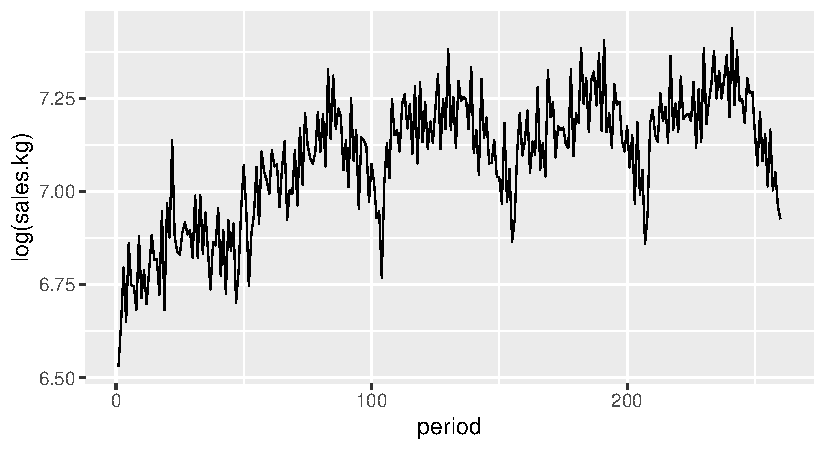
\includegraphics{tarea-eda-2_files/figure-latex/unnamed-chunk-3-1.pdf}

Usaremos suavizamiento con curvas loess para capturar los distintos
tipos de variación que observamos en la serie.

\begin{enumerate}
\def\labelenumi{\arabic{enumi}.}
\setcounter{enumi}{1}
\tightlist
\item
  Utiliza un suavizador \emph{loess} para capturar la tendencia de la
  serie.
\end{enumerate}

\begin{Shaded}
\begin{Highlighting}[]
\NormalTok{ajuste\_trend\_1 }\OtherTok{\textless{}{-}} \FunctionTok{loess}\NormalTok{(}\FunctionTok{log}\NormalTok{(sales.kg) }\SpecialCharTok{\textasciitilde{}}\NormalTok{ period, ventas, }\AttributeTok{span =} \FloatTok{0.5}\NormalTok{,}
                        \AttributeTok{degree =} \DecValTok{2}\NormalTok{)}

\NormalTok{ventas }\OtherTok{\textless{}{-}}\NormalTok{ ventas }\SpecialCharTok{|\textgreater{}} 
  \FunctionTok{add\_column}\NormalTok{(}\AttributeTok{trend\_1 =}\NormalTok{ ajuste\_trend\_1}\SpecialCharTok{$}\NormalTok{fitted,}
             \AttributeTok{res\_trend\_1 =}\NormalTok{ ajuste\_trend\_1}\SpecialCharTok{$}\NormalTok{residuals)}

               
\FunctionTok{ggplot}\NormalTok{(ventas, }\FunctionTok{aes}\NormalTok{(}\AttributeTok{x=}\NormalTok{period, }\AttributeTok{y=}\FunctionTok{log}\NormalTok{(sales.kg))) }\SpecialCharTok{+}
  \FunctionTok{geom\_line}\NormalTok{(}\AttributeTok{alpha =} \FloatTok{0.2}\NormalTok{) }\SpecialCharTok{+}
  \FunctionTok{geom\_line}\NormalTok{(}\FunctionTok{aes}\NormalTok{(}\AttributeTok{y =}\NormalTok{ trend\_1), }\AttributeTok{colour =} \StringTok{"red"}\NormalTok{, }\AttributeTok{size =} \FloatTok{1.2}\NormalTok{) }\SpecialCharTok{+} \FunctionTok{xlab}\NormalTok{(}\StringTok{"días"}\NormalTok{) }\SpecialCharTok{+}
  \FunctionTok{labs}\NormalTok{(}\AttributeTok{caption =} \StringTok{"Suavizamiento apropiado"}\NormalTok{)}
\end{Highlighting}
\end{Shaded}

\begin{verbatim}
## Warning: Using `size` aesthetic for lines was deprecated in ggplot2 3.4.0.
## i Please use `linewidth` instead.
## This warning is displayed once every 8 hours.
## Call `lifecycle::last_lifecycle_warnings()` to see where this warning was
## generated.
\end{verbatim}

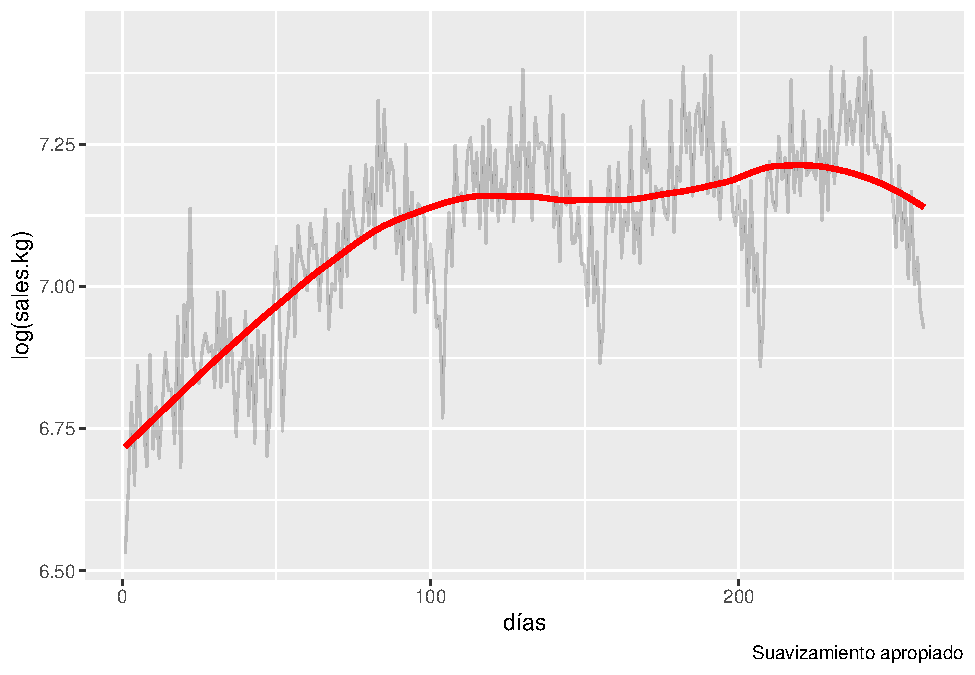
\includegraphics{tarea-eda-2_files/figure-latex/unnamed-chunk-4-1.pdf}

\begin{enumerate}
\def\labelenumi{\arabic{enumi}.}
\setcounter{enumi}{2}
\tightlist
\item
  Ahora calcula los residuales de este ajuste y descríbelos mediante un
  suavizamiento más fino. Verifica que se ha estimado la mayor parte de
  la tendencia, e intenta capturar la variación estacional de los
  residuales.
\end{enumerate}

CComo se puede observar, la variación estacional parece un seno. El
valor span = 0.2 da un buen resultado usando una relación cuadrática
(red line). Usando el valor de 0.1 para span (green line) todavía más
detallado. Un valor menos a span = 0.1 no llega a mejores resultados, y
mantiene más ruido.

\begin{Shaded}
\begin{Highlighting}[]
\NormalTok{periodic\_res2\_02 }\OtherTok{\textless{}{-}} \FunctionTok{loess}\NormalTok{(res\_trend\_1 }\SpecialCharTok{\textasciitilde{}}\NormalTok{ period, ventas, }\AttributeTok{span=}\FloatTok{0.2}\NormalTok{, }\AttributeTok{degree =} \DecValTok{2}\NormalTok{)}
\NormalTok{periodic\_res2\_01 }\OtherTok{\textless{}{-}} \FunctionTok{loess}\NormalTok{(res\_trend\_1 }\SpecialCharTok{\textasciitilde{}}\NormalTok{ period, ventas, }\AttributeTok{span=}\FloatTok{0.1}\NormalTok{, }\AttributeTok{degree =} \DecValTok{2}\NormalTok{)}

\NormalTok{g1 }\OtherTok{\textless{}{-}} \FunctionTok{ggplot}\NormalTok{(ventas, }\FunctionTok{aes}\NormalTok{(}\AttributeTok{x=}\NormalTok{period, }\AttributeTok{y=}\NormalTok{res\_trend\_1)) }\SpecialCharTok{+}
  \FunctionTok{geom\_line}\NormalTok{(}\AttributeTok{alpha =} \FloatTok{0.2}\NormalTok{) }\SpecialCharTok{+}
  \FunctionTok{geom\_line}\NormalTok{(}\FunctionTok{aes}\NormalTok{(}\AttributeTok{y =} \FunctionTok{fitted}\NormalTok{(periodic\_res2\_02)), }\AttributeTok{colour =} \StringTok{"red"}\NormalTok{, }\AttributeTok{size =} \FloatTok{1.2}\NormalTok{) }\SpecialCharTok{+}
  \FunctionTok{geom\_line}\NormalTok{(}\FunctionTok{aes}\NormalTok{(}\AttributeTok{y =} \FunctionTok{fitted}\NormalTok{(periodic\_res2\_01)), }\AttributeTok{colour =} \StringTok{"green"}\NormalTok{, }\AttributeTok{size =} \FloatTok{1.2}\NormalTok{) }
\NormalTok{periodic\_res2 }\OtherTok{\textless{}{-}}\NormalTok{ periodic\_res2\_01}
\NormalTok{g1}
\end{Highlighting}
\end{Shaded}

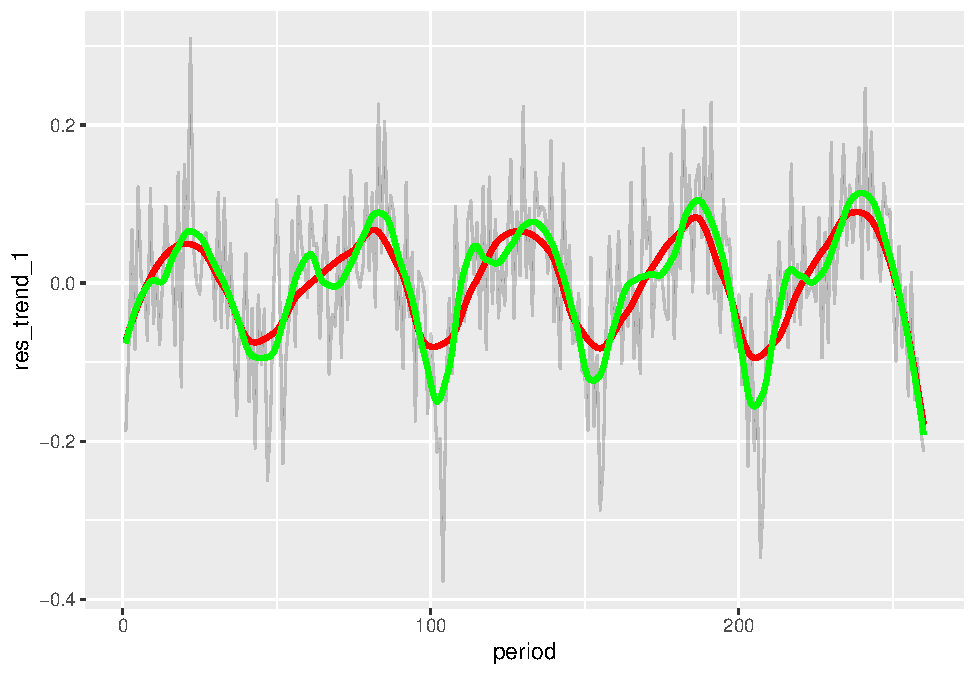
\includegraphics{tarea-eda-2_files/figure-latex/unnamed-chunk-5-1.pdf}

\begin{enumerate}
\def\labelenumi{\arabic{enumi}.}
\setcounter{enumi}{3}
\tightlist
\item
  Grafica los residuales obtenidos después de ajustar el componente
  estacional para estudiar la componente de mayor frecuencia.
\end{enumerate}

\begin{Shaded}
\begin{Highlighting}[]
\NormalTok{ventas }\OtherTok{\textless{}{-}}\NormalTok{ventas }\SpecialCharTok{|\textgreater{}} 
  \FunctionTok{add\_column}\NormalTok{(}\AttributeTok{periodic =}\NormalTok{ periodic\_res2}\SpecialCharTok{$}\NormalTok{fitted, }
             \AttributeTok{periodic\_res =}\NormalTok{ periodic\_res2}\SpecialCharTok{$}\NormalTok{residuals)}
\NormalTok{g2 }\OtherTok{\textless{}{-}} \FunctionTok{ggplot}\NormalTok{(ventas, }\FunctionTok{aes}\NormalTok{(}\AttributeTok{x=}\NormalTok{period, }\AttributeTok{y=}\NormalTok{periodic), }\AttributeTok{colour =} \StringTok{"green"}\NormalTok{, }\AttributeTok{size =} \FloatTok{1.0}\NormalTok{) }\SpecialCharTok{+}
  \FunctionTok{geom\_line}\NormalTok{(}\AttributeTok{alpha =} \FloatTok{0.2}\NormalTok{) }\SpecialCharTok{+}
  \FunctionTok{geom\_line}\NormalTok{(}\FunctionTok{aes}\NormalTok{(}\AttributeTok{y =}\NormalTok{ periodic\_res), }\AttributeTok{colour =} \StringTok{"red"}\NormalTok{, }\AttributeTok{size =} \FloatTok{0.8}\NormalTok{)}
\NormalTok{g2}
\end{Highlighting}
\end{Shaded}

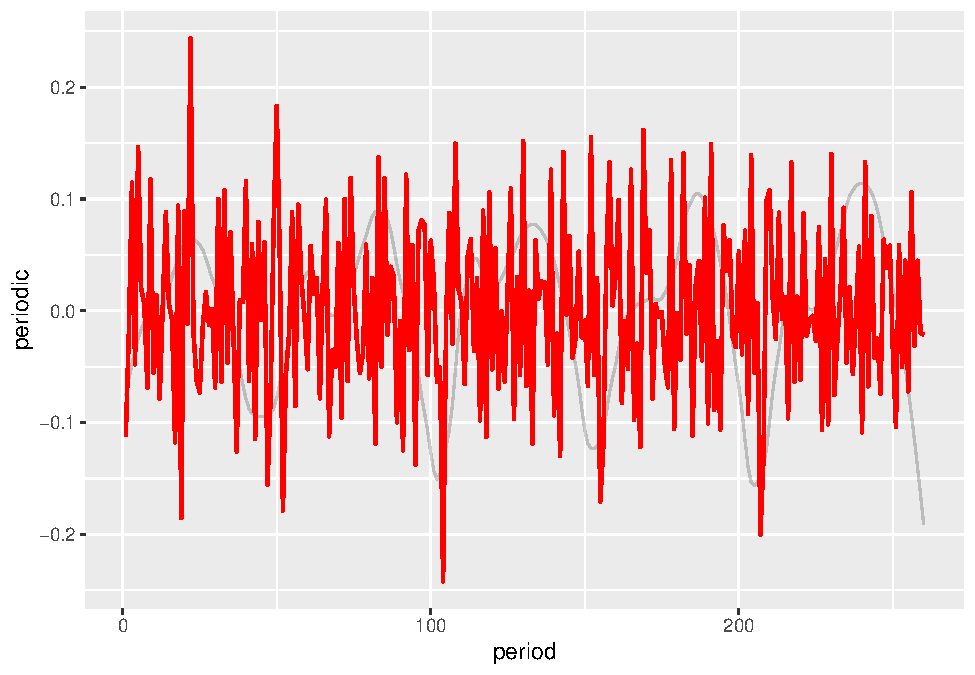
\includegraphics{tarea-eda-2_files/figure-latex/unnamed-chunk-6-1.pdf}

\begin{enumerate}
\def\labelenumi{\arabic{enumi}.}
\setcounter{enumi}{4}
\tightlist
\item
  (opcional) Visualiza el ajuste, genera una gráfica de páneles, en cada
  uno muestra una componente de la serie de tiempo y los residuales.
\end{enumerate}

\end{document}
